%
% IEEE Transactions on Microwave Theory and Techniques example
% Tibault Reveyrand - http://www.microwave.fr
%
% http://www.microwave.fr/LaTeX.html
% ---------------------------------------



% ================================================
% Please HIGHLIGHT the new inputs such like this :
% Text :
%  \hl{comment}
% Aligned Eq. 
% \begin{shaded}
% \end{shaded}
% ================================================



\documentclass[journal]{IEEEtran}

%\usepackage[retainorgcmds]{IEEEtrantools}
%\usepackage{bibentry}  
\usepackage{xcolor,soul,framed} %,caption

\colorlet{shadecolor}{yellow}
% \usepackage{color,soul}
\usepackage[pdftex]{graphicx}
\usepackage[]{algorithm2e}
\graphicspath{{../pdf/}{../jpeg/}}
\DeclareGraphicsExtensions{.pdf,.jpeg,.png}
\usepackage[cmex10]{amsmath}
%Mathabx do not work on ScribTex => Removed
%\usepackage{mathabx}
\usepackage{array}
\usepackage{mdwmath}
\usepackage{mdwtab}
\usepackage{eqparbox}
\usepackage{url}

%%%%%%%% Vu thêm %%%%%%%%%%%%%%%
\usepackage{amssymb, amsfonts}
% \usepackage{algorithm}
% \usepackage{algpseudocode}
% \usepackage{algcompatible}
% \usepackage[fleqn]{mathtools}
\usepackage[utf8]{vietnam}
%%%%%%%%%%%%%%%%%%%%%%%%%%%%%%%%%

\hyphenation{op-tical net-works semi-conduc-tor}

%\bstctlcite{IEEE:BSTcontrol}


%=== TITLE & AUTHORS ====================================================================
\begin{document}
\bstctlcite{IEEEexample:BSTcontrol}
    \title {Báo Cáo Đồ Án Cuối Kỳ CS116}
  \author{Huỳnh Hoàng Vũ - 20520864\,~\IEEEmembership{}\\
    CS116.O11.KHTN\\
      Đại học Công nghệ Thông tin\\% <-this % stops a space
      }


% The paper headers

\maketitle

% ====================================================================



% === ABSTRACT ====================================================================
% =================================================================================
% \begin{abstract}
% \end{abstract}


% === KEYWORDS ====================================================================
% =================================================================================
% \begin{IEEEkeywords}
% \hl{Reinforcement learning, Neural Network, Deep Reinforcement Learning}
% \end{IEEEkeywords}






% For peer review papers, you can put extra information on the cover
% page as needed:
% \ifCLASSOPTIONpeerreview
% \begin{center} \bfseries EDICS Category: 3-BBND \end{center}
% \fi
%
% For peerreview papers, this IEEEtran command inserts a page break and
% creates the second title. It will be ignored for other modes.
\IEEEpeerreviewmaketitle


% ====================================================================
% ====================================================================
% ====================================================================

\section{Giới thiệu bài toán}
Bộ dữ liệu Breast Cancer Wisconsin (Diagnostic) \cite{misc_breast_cancer_wisconsin_(diagnostic)_17} là một bộ dữ liệu phổ biến trong lĩnh vực học máy và phân loại. Bài toán liên quan đến việc dự đoán liệu một khối u vú là lành tính (benign) hay ác tính (malignant) dựa trên các đặc trưng y học của khối u.

Dữ liệu này chứa thông tin từ các phép đo của những tế bào trong các khối u vú và được sử dụng để xây dựng các mô hình học máy có khả năng dự đoán xác suất của việc u lành tính hoặc ác tính. Mỗi mẫu trong bộ dữ liệu bao gồm các đặc trưng hình ảnh như bán kính, diện tích, độ đo đồng nhất, độ đo độ lệch và nhiều thông số khác.

Đây là một bài toán phân loại hai lớp (binary classification) phổ biến trong lĩnh vực y học và có thể áp dụng nhiều phương pháp học máy như Support Vector Machine (SVM), Decision Tree, Random Forest, Deep Neural Network và các mô hình phân loại khác.

Mục tiêu của bài toán này là xây dựng một mô hình học máy có khả năng dự đoán xác suất hoặc lớp (benign/malignant) của khối u vú dựa trên các đặc trưng hóa học của nó. Điều này có thể giúp các chuyên gia y tế đưa ra quyết định về liệu pháp điều trị và quản lý bệnh nhân.

\section{Phân tích dữ liệu khám phá (EDA)}
dataprep.eda \cite{dataprepeda2021} là một công cụ hữu ích giúp tự động phân tích dữ liệu khám phá (Automated EDA). Với hàm create\_report giúp ta có một cái nhìn tổng quan về dữ liệu. Hình \ref{fig:correlation} và Hình \ref{fig:missing} lần lượt thể hiện thông tin độ tương quan giữa các cột và thông tin dữ liệu bị thiếu sử dụng thư viện dataprep. Ta có thể thấy dữ liệu khá đầy đủ khi không có giá trị thiếu nào. Trong khi đó, nhiều có sự tương quan mạnh với nhau.

\begin{figure}
    \centering
    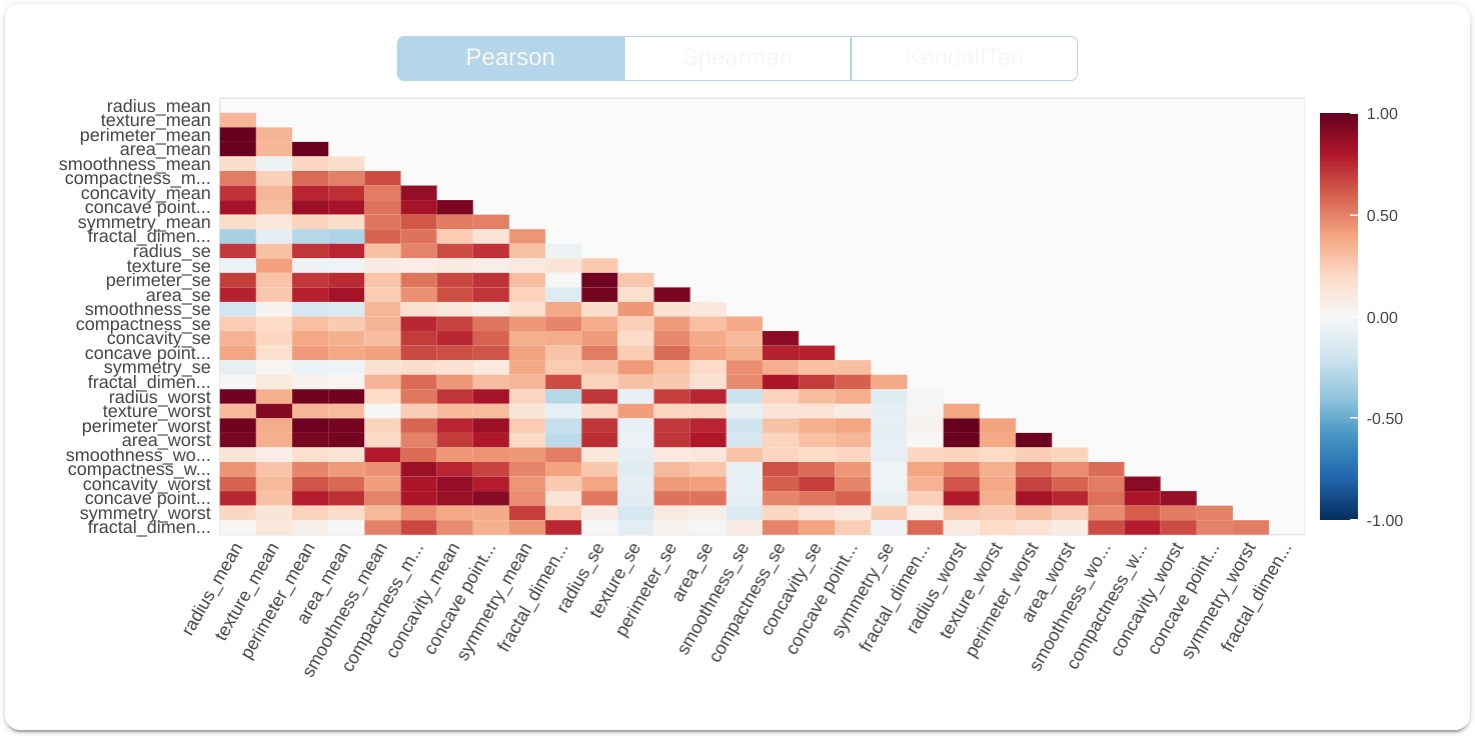
\includegraphics[width=\linewidth]{img/correlation.jpeg}
    \caption{Thông tin độ tương quan giữa các cột sử dụng thư viện dataprep.}
    \label{fig:correlation}
\end{figure}
\begin{figure}
    \centering
    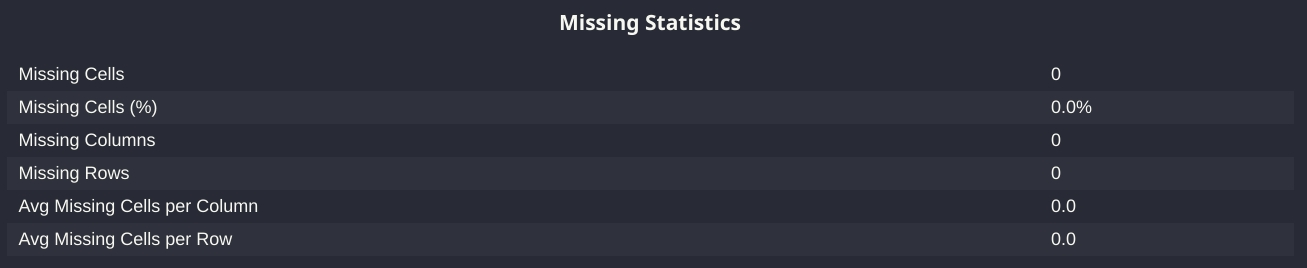
\includegraphics[width=\linewidth]{img/missing.jpeg}
    \caption{Thông tin dữ liệu bị thiếu sử dụng thư viện dataprep.}
    \label{fig:missing}
\end{figure}

\section{Chuẩn bị dữ liệu}
Trước hết, cột target "diagnosis" là nhãn cần được phân loại cần được mã hóa từ dạng chuỗi sang dạng số bằng class LabelEncoder của thư viện scikit-learn \cite{scikit-learn}.
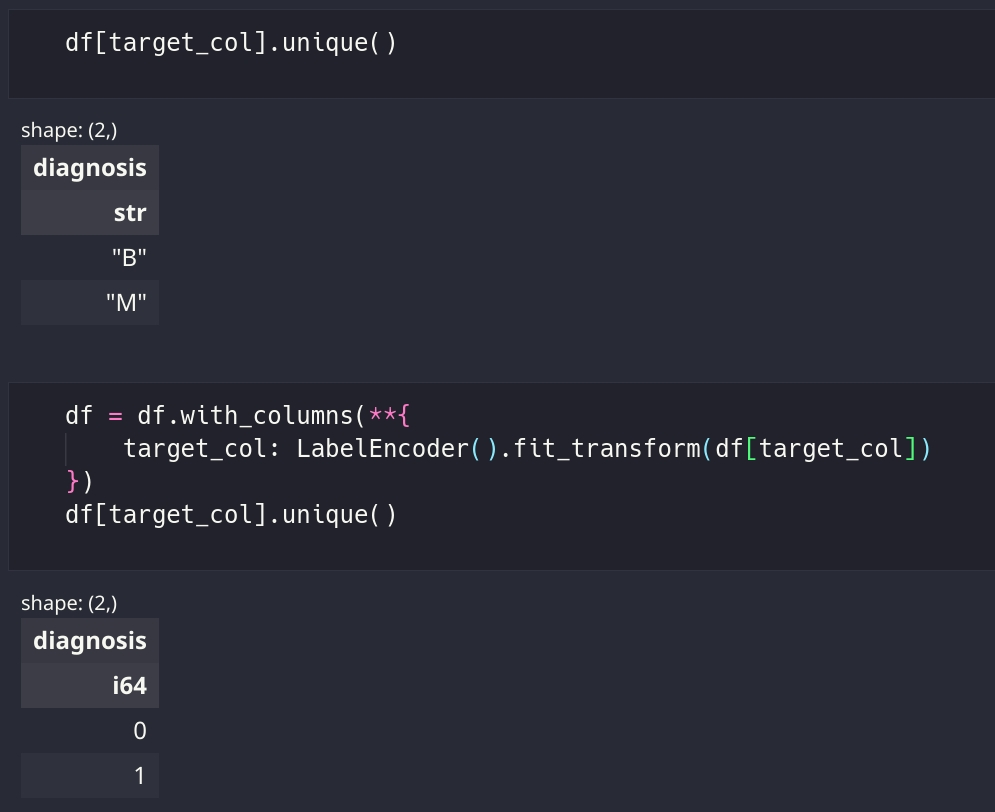
\includegraphics[width=\linewidth]{img/encode.jpeg}
% \begin{figure}[h]
%     \centering
%     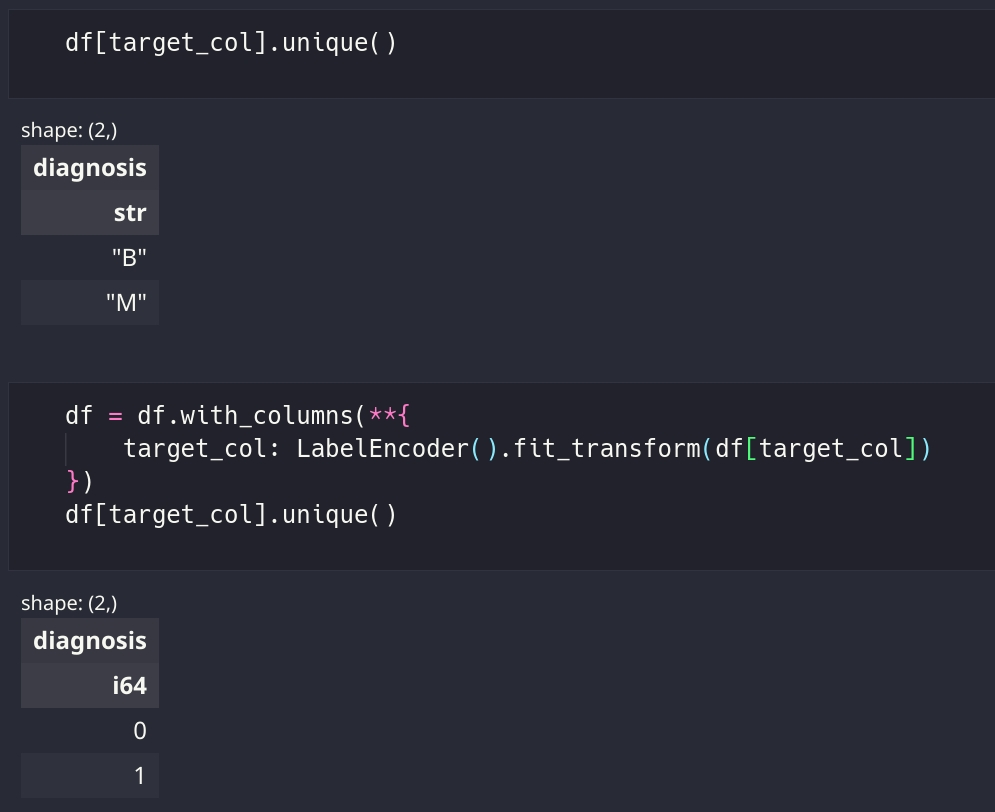
\includegraphics[width=\linewidth]{img/encode.jpeg}
%     \label{fig:encode}
% \end{figure}

Sau khi mã hóa, về cơ bản, dữ liệu đã đúng định dạng để đưa vào các mô hình máy học. Em đặt tên bộ dữ liệu sau khi được mã hóa là "orginal". Bên cạnh đó, em còn thực hiện ba phép biến đổi khác từ bộ dữ liệu orginal, được đặt tên lần lượt là "random\_corr\_remove", "ordered\_corr\_remove", "pca". Cả random\_corr\_remove và ordered\_corr\_remove đều là phép loại bỏ các đặc trưng có độ tương quan cao. Điểm khác nhau duy nhất là random\_corr\_remove xem xét loại bỏ các đặc trưng theo thứ tự ngẫu nhiên, còn ordered\_corr\_remove thì ưu tiên loại bỏ các đặc trưng tương quan yếu với target (Hình \ref{fig:corr}).
\begin{figure*}
    \centering
    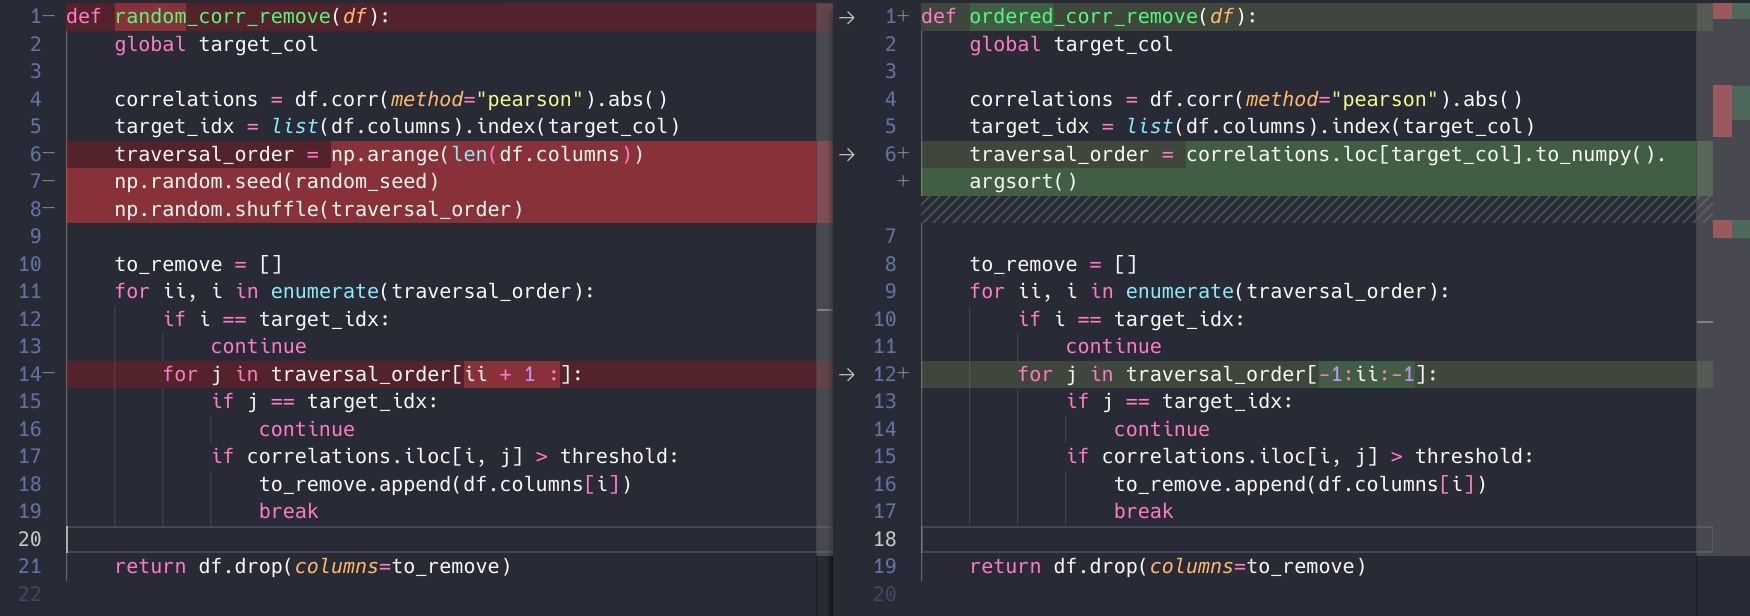
\includegraphics[width=\linewidth]{img/corr.jpeg}
    \caption {Sự khác nhau giữa random\_corr\_remove và ordered\_corr\_remove trong cài đặt.}
    \label{fig:corr}
\end{figure*}
% \begin{figure}[h]
%     \centering
%     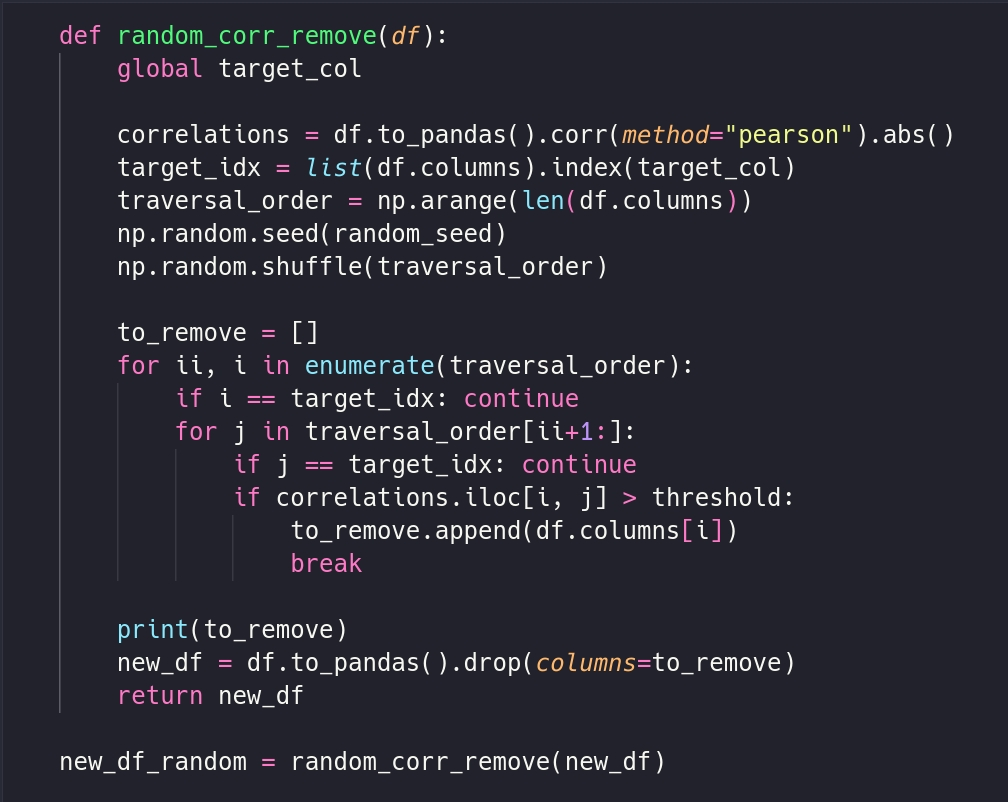
\includegraphics[width=\linewidth]{img/rand_corr.jpeg}
%     \label{fig:rand_corr}
% \end{figure}
% \begin{figure}[h]
%     \centering
%     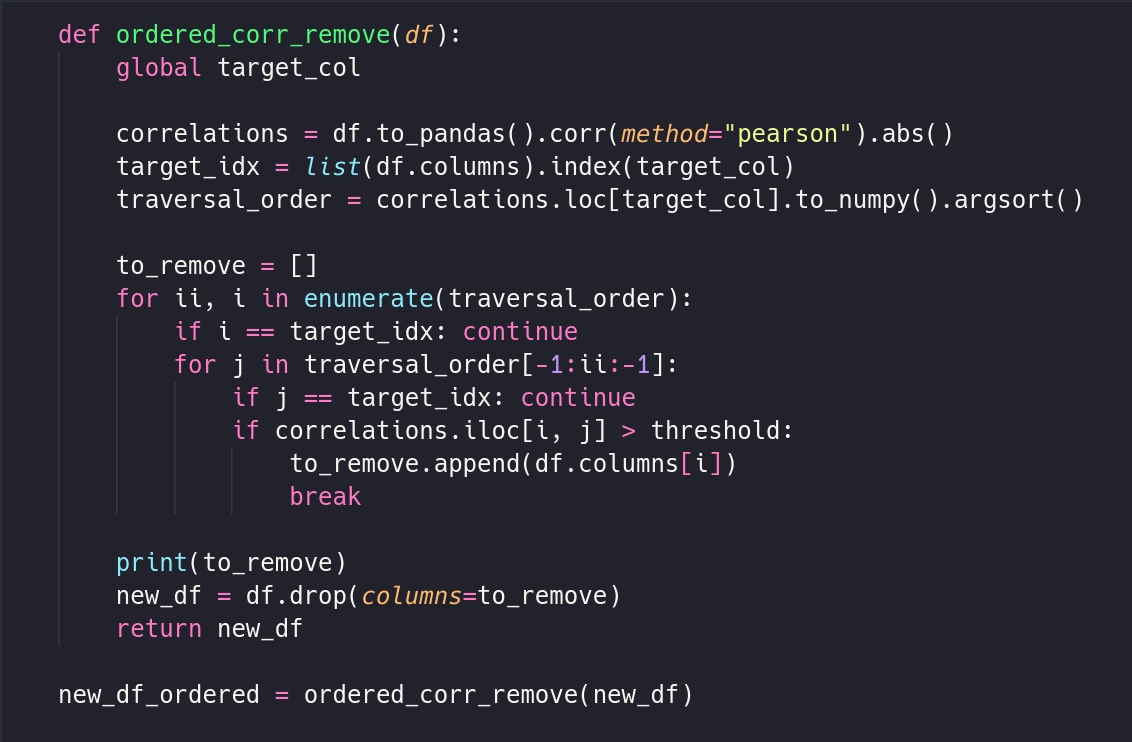
\includegraphics[width=\linewidth]{img/ord_corr.jpeg}
%     \label{fig:ord_corr}
% \end{figure}
Với bộ dữ liệu pca, em dùng class PCA của scikit-learn để giảm số đặc trưng của dữ liệu.

\section {Thiết kế thực nghiệm}
Để có một kết quả ít bị thiên lệch, em sử dụng 5-fold cross-validation.
Thang đo được dùng đến là accuracy.
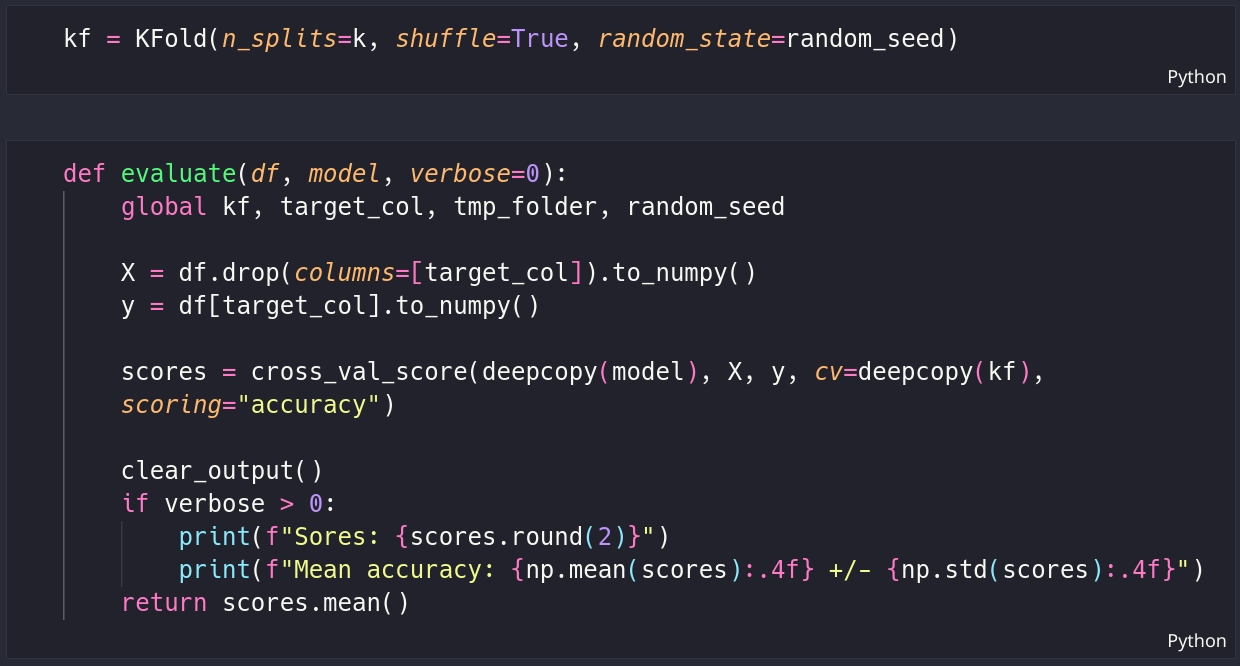
\includegraphics[width=\linewidth]{img/cross_val.jpeg}
% \begin{figure}[h]
%     \centering
%     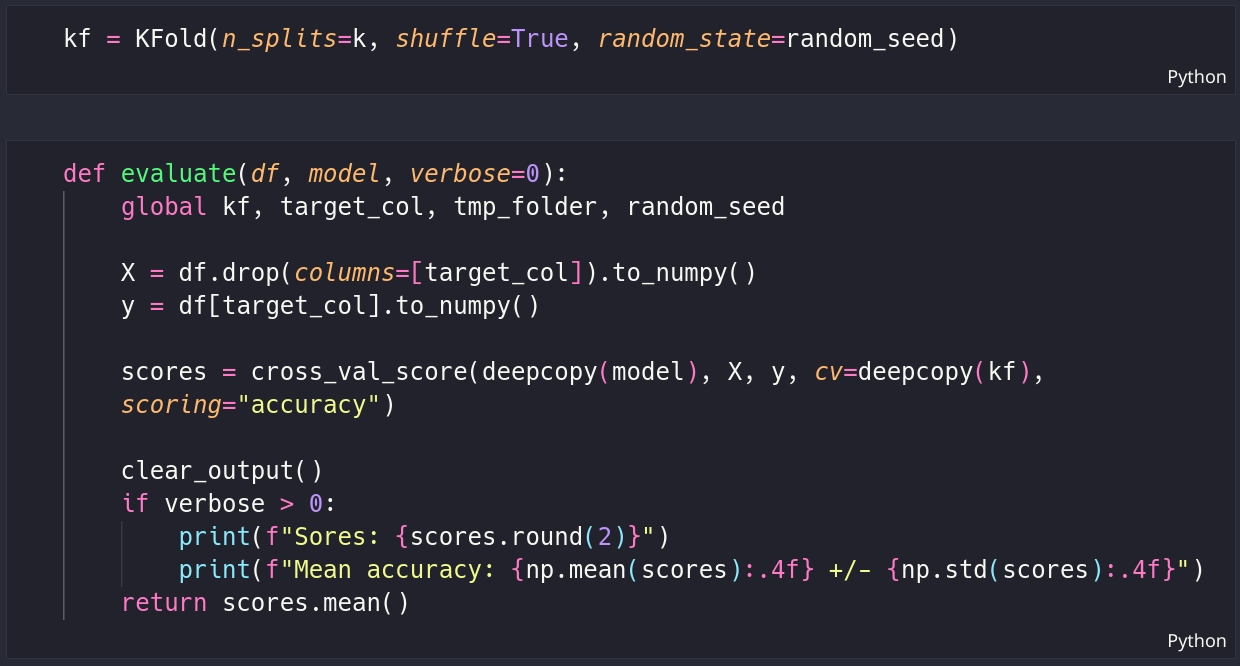
\includegraphics[width=\linewidth]{img/cross_val.jpeg}
%     \label{fig:cross_val}
% \end{figure}
Thực nghiệm tiến hành so sánh thuật toán TabPFN \cite{hollmann2023tabpfn} và XGBoost \cite{Chen2016} với phiên bản có Cleanlab \cite{northcutt2021confidentlearning} bọc bên ngoài hoặc không. Đồng thời, so sánh tính hiệu quả của các cách tiền xử lý dữ liệu.
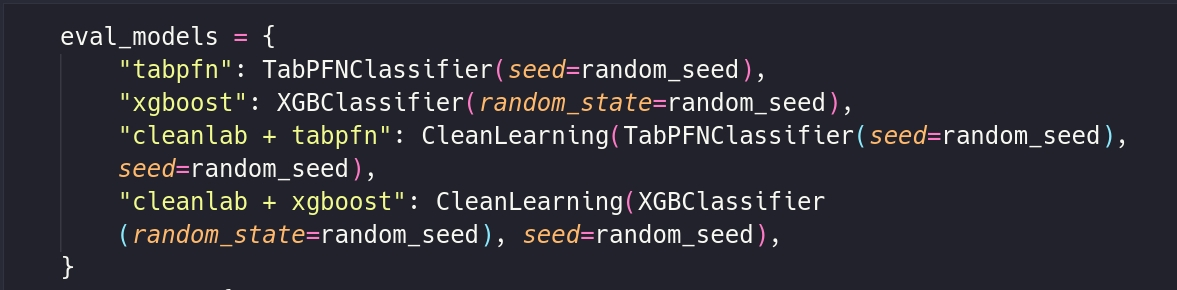
\includegraphics[width=\linewidth]{img/models.jpeg}
% \begin{figure}[h]
%     \centering
%     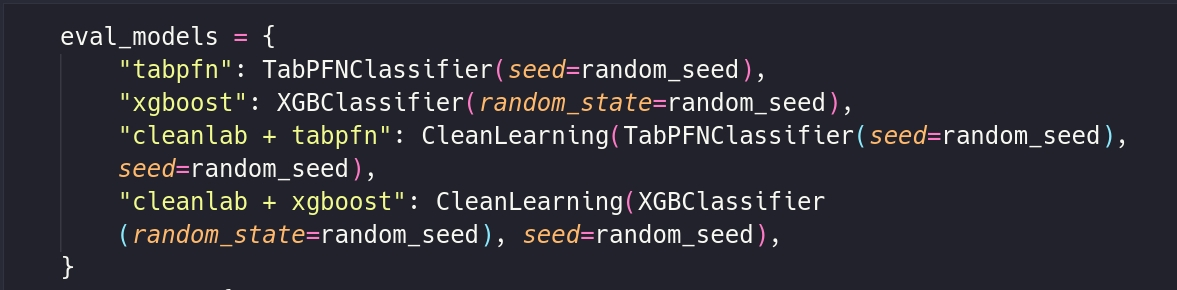
\includegraphics[width=\linewidth]{img/models.jpeg}
%     \label{fig:models}
% \end{figure}

\section {Kết quả thực nghiệm}
\begin{table*}
    \centering
    \begin{tabular}{c|c|c|c|c}
         & tabpfn & xgboost & cleanlab + tabpfn & cleanlab + xgboost \\
        \hline
        original & 0.962857 & \textbf{0.974286} & 0.948571 & 0.954286 \\
        \hline
        random\_corr\_remove & 0.96 & 0.957143 & 0.954286 & 0.925714 \\
        \hline
        ordered\_corr\_remove & 0.965714 & 0.965714 & 0.957143 & 0.954286 \\
        \hline
        pca & 0.945714 & 0.937143 & 0.954286 & 0.931429
    \end{tabular}
    \caption{Hiệu suất của các cách tiền xử lý ứng với các thuật toán.}
    \label{tab:performance}
\end{table*}
Dựa vào Bảng \ref{tab:performance}, trên dataframe gốc, ta có thể thấy sử dụng thuật toán XGBoost mang lại độ chính xác cao nhất 97\%, kế đến là TabPFN 96\%. Đáng ngạc nhiên là ở các dataframe khác TabPFN lại cho độ chính xác cao nhất. Cleanlab không thực sự giúp ích trong thực nghiệm này, khi mà nó làm giảm độ chính xác của thuật toán gốc ở phần lớn các trường hợp (trừ Cleanlab+TabPFN với PCA).

Quan sát các cách tiền xử lý, nhìn chung, PCA mang lại kết quả tệ hơn 2 phép biến đổi còn lại. random\_corr\_remove hơn điểm dataframe gốc 1 lần, PCA hơn 1 lần, orderd\_corr\_remove hơn 2 lần cho thấy các cách tiền xử lý trên không thực sự hiệu quả, đặc biệt là với XGBoost.

Khi so sánh 2 kiểu lượt bỏ các đặc trưng tương quan mạnh, 1 là duyệt theo thứ tự ngẫu nhiên random\_corr\_remove, 2 là duyệt theo thứ tự xác định orderd\_corr\_remove, orderd\_corr\_remove mang lại kết quả tốt hơn hẳn. Ta có thể kết luận, việc ưu tiên loại bỏ đặc trưng tương quan yếu với target, giữ lại đặc trưng tương quan mạnh với target là tốt hơn so với việc không quan tâm yếu tố này.


% ===================================================================================================================================


% An example of a floating figure using the graphicx package.
% Note that \label must occur AFTER (or within) \caption.
% For figures, \caption should occur after the \includegraphics.
% Note that IEEEtran v1.7 and later has special internal code that
% is designed to preserve the operation of \label within \caption
% even when the captionsoff option is in effect. However, because
% of issues like this, it may be the safest practice to put all your
% \label just after \caption rather than within \caption{}.
%
% Reminder: the "draftcls" or "draftclsnofoot", not "draft", class
% option should be used if it is desired that the figures are to be
% displayed while in draft mode.
%
%\begin{figure}[!t]
%\centering
%\includegraphics[width=2.5in]{myfigure}
% where an .eps filename suffix will be assumed under latex, 
% and a .pdf suffix will be assumed for pdflatex; or what has been declared
% via \DeclareGraphicsExtensions.
%\caption{Simulation Results}
%\label{fig_sim}
%\end{figure}

% Note that IEEE typically puts floats only at the top, even when this
% results in a large percentage of a column being occupied by floats.


% An example of a double column floating figure using two subfigures.
% (The subfig.sty package must be loaded for this to work.)
% The subfigure \label commands are set within each subfloat command, the
% \label for the overall figure must come after \caption.
% \hfil must be used as a separator to get equal spacing.
% The subfigure.sty package works much the same way, except \subfigure is
% used instead of \subfloat.
%
%\begin{figure*}[!t]
%\centerline{\subfloat[Case I]\includegraphics[width=2.5in]{subfigcase1}%
%\label{fig_first_case}}
%\hfil
%\subfloat[Case II]{\includegraphics[width=2.5in]{subfigcase2}%
%\label{fig_second_case}}}
%\caption{Simulation results}
%\label{fig_sim}
%\end{figure*}
%
% Note that often IEEE papers with subfigures do not employ subfigure
% captions (using the optional argument to \subfloat), but instead will
% reference/describe all of them (a), (b), etc., within the main caption.


% An example of a floating table. Note that, for IEEE style tables, the 
% \caption command should come BEFORE the table. Table text will default to
% \footnotesize as IEEE normally uses this smaller font for tables.
% The \label must come after \caption as always.
%
%\begin{table}[!t]
%% increase table row spacing, adjust to taste
%\renewcommand{\arraystretch}{1.3}
% if using array.sty, it might be a good idea to tweak the value of
% \extrarowheight as needed to properly center the text within the cells
%\caption{An Example of a Table}
%\label{table_example}
%\centering
%% Some packages, such as MDW tools, offer better commands for making tables
%% than the plain LaTeX2e tabular which is used here.
%\begin{tabular}{|c||c|}
%\hline
%One & Two\\
%\hline
%Three & Four\\
%\hline
%\end{tabular}
%\end{table}


% Note that IEEE does not put floats in the very first column - or typically
% anywhere on the first page for that matter. Also, in-text middle ("here")
% positioning is not used. Most IEEE journals use top floats exclusively.
% Note that, LaTeX2e, unlike IEEE journals, places footnotes above bottom
% floats. This can be corrected via the \fnbelowfloat command of the
% stfloats package.





% if have a single appendix:
%\appendix[Proof of the Zonklar Equations]
% or
%\appendix  % for no appendix heading
% do not use \section anymore after \appendix, only \section*
% is possibly needed

% use appendices with more than one appendix
% then use \section to start each appendix
% you must declare a \section before using any
% \subsection or using \label (\appendices by itself
% starts a section numbered zero.)
%

% ============================================
%\appendices
%\section{Proof of the First Zonklar Equation}
%Appendix one text goes here %\cite{Roberg2010}.

% you can choose not to have a title for an appendix
% if you want by leaving the argument blank
%\section{}
%Appendix two text goes here.


% use section* for acknowledgement
%\section*{Acknowledgment}


%The authors would like to thank D. Root for the loan of the SWAP. The SWAP that can ONLY be usefull in Boulder...


% Can use something like this to put references on a page
% by themselves when using endfloat and the captionsoff option.
\ifCLASSOPTIONcaptionsoff
  \newpage
\fi



% trigger a \newpage just before the given reference
% number - used to balance the columns on the last page
% adjust value as needed - may need to be readjusted if
% the document is modified later
%\IEEEtriggeratref{8}
% The "triggered" command can be changed if desired:
%\IEEEtriggercmd{\enlargethispage{-5in}}

% ====== REFERENCE SECTION

%\begin{thebibliography}{1}

% IEEEabrv,

\bibliographystyle{IEEEtran}
\bibliography{IEEEabrv,Bibliography}
%\end{thebibliography}
% biography section
% 
% If you have an EPS/PDF photo (graphicx package needed) extra braces are
% needed around the contents of the optional argument to biography to prevent
% the LaTeX parser from getting confused when it sees the complicated
% \includegraphics command within an optional argument. (You could create
% your own custom macro containing the \includegraphics command to make things
% simpler here.)
%\begin{biography}[{\includegraphics[width=1in,height=1.25in,clip,keepaspectratio]{mshell}}]{Michael Shell}
% or if you just want to reserve a space for a photo:

% ==== SWITCH OFF the BIO for submission
% ==== SWITCH OFF the BIO for submission
% \begin{IEEEbiography}[{\includegraphics[width=1in,height=1.25in,clip,keepaspectratio]{photo/mike.png}}]{Michael Roberg}
% (S'09) received the B.S.E.E degree from Bucknell University, Lewisburg, PA, in 2003, the M.S.E.E. degree from the University of Pennsylvania, Philadelphia, in 2006, and the Ph.D. degree from the University of Colorado at Boulder in 2012. From 2003 to 2009, he was an Engineer with Lockheed Martin–MS2, Moorestown, NJ, where he was involved with advanced phased-array radar systems. His current research interests include high efficiency microwave PA theory and design, microwave power rectifiers, MMIC design, and high-efficiency radar and communication system transmitters. He is currently employed by TriQuint Semiconductor - Defense Products and Foundry Services in Richardson, TX working on wideband high efficiency GaN MMIC PA design.
% \end{IEEEbiography}
% \begin{IEEEbiography}[{\includegraphics[width=1in,height=1.25in,clip,keepaspectratio]{photo/tibo.png}}]{Tibault Reveyrand}
% (M'07)  received the Ph.D. degree from the University of Limoges, France, in 2002.
% From 2002 to 2004, he was a Post-Doctoral Scientist with CNES (French Space Agency). In 2005, he became a CNRS engineer at XLIM. His research interests include the characterization and modeling of RF and microwave nonlinear components and devices.
% Dr. Reveyrand was the recipient of the 2002 European GaAs Best Paper Award and is a member of the IEEE MTT-11 "Microwave Measurements" Technical Committee.
% \end{IEEEbiography}
% \begin{IEEEbiography}[{\includegraphics[width=1in,height=1.25in,clip,keepaspectratio]{photo/ignacio.png}}]{Ignacio Ramos}
% (S'12) received the B.S. degree in electrical engineering from the University of Illinois at Chicago in 2009, and is currently working toward the Ph.D. degree at the University of Colorado at Boulder. From 2009 to 2011, he was with the Power and Electronic Systems Department at Raytheon IDS, Sudbury, MA. His research interests include high-efficiency microwave power amplifiers, microwave DC/DC converters, radar systems, and wireless power transmission.
% \end{IEEEbiography}
% \begin{IEEEbiography}[{\includegraphics[width=1in,height=1.25in,clip,keepaspectratio]{photo/erez.png}}]{Erez Avigdor Falkenstein}
% (S'07), Haifa, Israel in 1979. He earned a “Handesaie” degree (associate degree) in electronics from Amal Handesaim School Hadera, Israel in 1999. From 1999 to 2003 he served in the Israel Defense Force as part of a technological unit. He has been at the University of Colorado at Boulder 2004 – 2012. He received concurrent MS/BS degrees in Electrical engineering 2010 and a Ph.D 2012 from the University of Colorado at Boulder. Since 2007 he has been involved with research as part of the active antenna group. Research emphasis: far field wireless powering for low power densities. Interests include Antenna design and characterization, modeling and measurement of nonlinear devices at microwave frequencies and power management. He is currently employed at Qualcomm, Incorporated, Boulder, CO.
% \end{IEEEbiography}
% \begin{IEEEbiography}[{\includegraphics[width=1in,height=1.25in,clip,keepaspectratio]{photo/zoya.png}}]{Zoya Popovi\'c}
% (S'86-M'90-SM'99-F'02) received the Dipl.Ing. degree from the University of Belgrade, Belgrade, Serbia, Yugoslavia, in 1985, and the Ph.D. degree from the California Institute of Technology, Pasadena, in 1990.
% Since 1990, she has been with the University of Colorado at Boulder, where she is currently a Distinguished Professor and holds the Hudson Moore Jr. Chair with the Department of Electrical, Computer and Energy Engineering. In 2001, she was a Visiting Professor with the Technical University of Munich, Munich, Germany. 
% Since 1991, she has graduated 44 Ph.D. students. Her research interests include high-efficiency, low-noise, and broadband microwave and millimeter-wave circuits, quasi-optical millimeter-wave techniques, active
% antenna arrays, and wireless powering for batteryless sensors.
% Prof. Popovi\'c was the recipient of the 1993 and 2006 Microwave Prizes presented by the IEEE Microwave Theory and Techniques Society (IEEE MTT-S) for the best journal papers and the 1996 URSI Issac Koga Gold Medal. In 1997, Eta Kappa Nu students chose her as a Professor of the Year. She was the recipient of a 2000 Humboldt Research Award for Senior U.S. Scientists of the German Alexander von Humboldt Stiftung. She was elected a Foreign Member of the Serbian Academy of Sciences and Arts in 2006. She was also the recipient of the 2001 Hewlett-Packard (HP)/American Society for Engineering Education (ASEE) Terman Medal for combined teaching and research excellence.
% \end{IEEEbiography}

%% if you will not have a photo at all:
%\begin{IEEEbiographynophoto}{Ignacio Ramos}
%(S'12) received the B.S. degree in electrical engineering from the University of Illinois at Chicago in 2009, and is currently working toward the Ph.D. degree at the University of Colorado at Boulder. From 2009 to 2011, he was with the Power and Electronic Systems Department at Raytheon IDS, Sudbury, MA. His research interests include high-efficiency microwave power amplifiers, microwave DC/DC converters, radar systems, and wireless power transmission.
%\end{IEEEbiographynophoto}


%% insert where needed to balance the two columns on the last page with
%% biographies
%%\newpage

%\begin{IEEEbiographynophoto}{Jane Doe}
%Biography text here.
%\end{IEEEbiographynophoto}
% ==== SWITCH OFF the BIO for submission
% ==== SWITCH OFF the BIO for submission



% You can push biographies down or up by placing
% a \vfill before or after them. The appropriate
% use of \vfill depends on what kind of text is
% on the last page and whether or not the columns
% are being equalized.

\vfill

% Can be used to pull up biographies so that the bottom of the last one
% is flush with the other column.
%\enlargethispage{-5in}



% that's all folks
\end{document}


